\documentclass[aspectratio=169,10pt]{beamer}
\usetheme{Madrid}
\usecolortheme{default}

\usepackage[utf8]{inputenc}
\usepackage{booktabs}
\usepackage{amsmath}
\usepackage{array}
\usepackage{graphicx}
\usepackage{tikz}
\usepackage{hyperref}

\title[TDA Landscapes of Crashes]{Replication of \\ Topological Data Analysis of Financial Time Series: Landscapes of Crashes}
\subtitle{Statistics 565 - Final Presentation}
\author{Artem Ivaniuk}
\date{\today}

\begin{document}

\begin{frame}
  \titlepage
\end{frame}

\begin{frame}{Research Question}
\textbf{Paper:} Gidea $\&$ Katz (2017), \emph{Topological Data Analysis of Financial Time Series: Landscapes of Crashes}

\vspace{0.5em}
\textbf{Core question:} Can we use topology to detect financial crises before they happen?

\vspace{0.5em}
\textbf{Why this is interesting:}
\begin{itemize}
  \item Goes beyond standard volatility/correlation diagnostics 
  \item Uses shape-based features of data clouds, not only moments (i.e. mean, variance, etc.)
  \item Tests whether geometry/topology captures regime shifts before crashes
\end{itemize}
\end{frame}

\begin{frame}{Replication Setup}
\textbf{Source:} Yahoo Finance daily adjusted close data
\begin{itemize}
  \item S\&P 500 (\texttt{\^{}GSPC}), DJIA (\texttt{\^{}DJI}), NASDAQ (\texttt{\^{}IXIC}), Russell 2000 (\texttt{\^{}RUT})
  \item VIX (\texttt{\^{}VIX}) used as benchmark comparison signal
\end{itemize}

\vspace{0.4em}
\textbf{Replication sample}
\begin{itemize}
  \item Raw prices pulled over 1987-12-23 to 2016-12-08 (pipeline-aligned)
  \item Effective return sample in notebook: 1992-01-03 to 2016-12-08
  \item Working matrix: 4D daily log returns
\end{itemize}

\vspace{0.4em}
\[
r_{i,j} = \log\!\left(\frac{P_{i,j}}{P_{i-1,j}}\right)
\]
\end{frame}

\begin{frame}{Data Geometry View}
\textbf{Object of interest:} rolling \emph{clouds} of multivariate returns, not a single series
\begin{itemize}
  \item At each date \(t\), take the most recent \(w\in\{50,100\}\) days of 4-index returns.
  \item This gives a point cloud \(X_t\subset\mathbb{R}^4\): one point per day, four coordinates per point.
  \item We ask how the cloud's \emph{shape} changes as markets move from calm to stress.
\end{itemize}

\vspace{0.4em}
\textbf{Why this setup is sensible}
\begin{itemize}
  \item Crises are multivariate phenomena (co-movement, dispersion, nonlinear interaction).
  \item Shape-based summaries can capture structure missed by mean/variance alone.
  \item Rolling windows let the geometry evolve through time, enabling early-warning tracking.
\end{itemize}
\end{frame}

\begin{frame}{Topological Pipeline}
\textbf{Step 1: Persistent homology on each cloud}
\begin{itemize}
  \item Build Vietoris--Rips complexes as radius \(\epsilon\) grows.
  \item Track \(H_1\) features (loops): birth/death pairs \((b_k,d_k)\).
  \item Output: persistence diagram \(D_t^{(1)}\) for each date \(t\).
\end{itemize}

\textbf{Step 2: Convert to stable numeric summaries}
\begin{itemize}
  \item Transform each diagram into a persistence landscape \(\lambda_t\).
  \item Compute \(\|\lambda_t\|_1\) and \(\|\lambda_t\|_2\).
  \item Output: two time series of topological ``market stress'' indicators.
\end{itemize}

\textbf{Step 3: Early-warning diagnostics}
\begin{itemize}
  \item Rolling variance and low-frequency PSD of \(L_1\) norm.
  \item Kendall \(\tau\) trend tests on pre-crash windows.
\end{itemize}
\end{frame}

\begin{frame}{Quick Topology Guide}
\textbf{Point cloud \(X_t\)}
\begin{itemize}
  \item A set of points in \(\mathbb{R}^4\): each point is one trading day of 4-index returns.
\end{itemize}

\textbf{Vietoris--Rips complex (scale \(\epsilon\))}
\begin{itemize}
  \item Connect points that are within distance \(\epsilon\); this builds a network/shape proxy.
  \item Increase \(\epsilon\) to see how connectivity and loops appear/disappear.
\end{itemize}

\textbf{Persistent homology (\(H_1\))}
\begin{itemize}
  \item Tracks loop features through scales; each has birth \(b\) and death \(d\).
  \item \textbf{Birth \(b\):} the first scale where a loop appears in the Rips complex.
  \item \textbf{Death \(d\):} the scale where that loop gets filled in/merged and no longer exists.
  \item \textbf{Lifetime \(d-b\):} persistence of that feature across scales.
  \item Short lifetimes are typically local noise; long lifetimes are stable global structure.
  \item Output is a persistence diagram (all \((b,d)\) pairs), then landscape norms that summarize overall topological complexity over time.
\end{itemize}
\end{frame}

\begin{frame}{Why Do This}
\textbf{Why not just variance/correlation?}
\begin{itemize}
  \item Those are low-order summaries; they can miss changes in multivariate geometry.
  \item Crisis buildup can alter cloud \emph{shape} before level/volatility fully breaks.
\end{itemize}

\textbf{What the topological map gives us}
\begin{itemize}
  \item For each date \(t\): a persistence diagram \(D_t^{(1)}\) (all loop lifetimes at once).
  \item A stable functional form \(\lambda_t\) (persistence landscape) for computation/comparison.
  \item Scalar indicators \(\|\lambda_t\|_1,\|\lambda_t\|_2\) that become time-series risk signals.
  \item Testable outputs: trend statistics, event-window comparisons, and cross-signal checks vs VIX.
\end{itemize}
\end{frame}

\begin{frame}{Persistence Diagram and Landscape (Graphic)}
\begin{columns}[T,onlytextwidth]
\column{0.49\textwidth}
\centering
\textbf{Persistence diagram \(D_t^{(1)}\)}\\[0.2em]
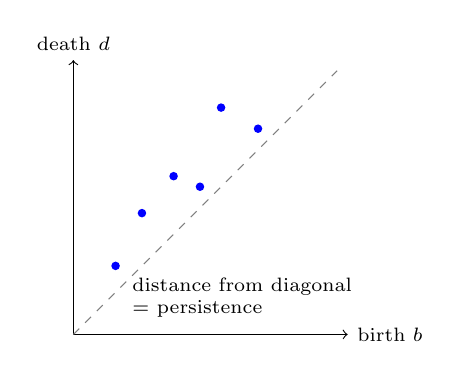
\begin{tikzpicture}[scale=0.67]
  \draw[->] (0,0) -- (5.2,0) node[right] {\scriptsize birth \(b\)};
  \draw[->] (0,0) -- (0,5.2) node[above] {\scriptsize death \(d\)};
  \draw[dashed,gray] (0,0) -- (5,5);
  \fill[blue] (0.8,1.3) circle (2.3pt);
  \fill[blue] (1.3,2.3) circle (2.3pt);
  \fill[blue] (1.9,3.0) circle (2.3pt);
  \fill[blue] (2.4,2.8) circle (2.3pt);
  \fill[blue] (2.8,4.3) circle (2.3pt);
  \fill[blue] (3.5,3.9) circle (2.3pt);
  \node[align=left,font=\scriptsize] at (3.2,0.7) {distance from diagonal\\= persistence};
\end{tikzpicture}

\column{0.49\textwidth}
\centering
\textbf{Persistence landscape \(\lambda_t\)}\\[0.2em]
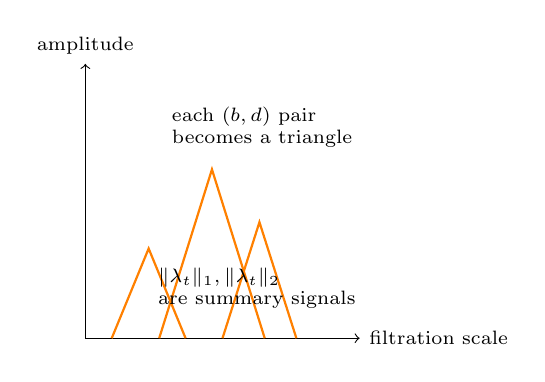
\begin{tikzpicture}[scale=0.67]
  \draw[->] (0,0) -- (5.2,0) node[right] {\scriptsize filtration scale};
  \draw[->] (0,0) -- (0,5.2) node[above] {\scriptsize amplitude};
  \draw[thick,orange] (0.5,0) -- (1.2,1.7) -- (1.9,0);
  \draw[thick,orange] (1.4,0) -- (2.4,3.2) -- (3.4,0);
  \draw[thick,orange] (2.6,0) -- (3.3,2.2) -- (4.0,0);
  \node[align=left,font=\scriptsize] at (3.35,4.0) {each \((b,d)\) pair\\becomes a triangle};
  \node[align=left,font=\scriptsize] at (3.25,0.95) {\(\|\lambda_t\|_1,\|\lambda_t\|_2\)\\are summary signals};
\end{tikzpicture}
\end{columns}

\vspace{0.3em}
\footnotesize
Left: raw topological features. Right: smooth representation used to compare windows and build risk-indicator time series.
\end{frame}

\begin{frame}{Input Data Snapshot}
\centering
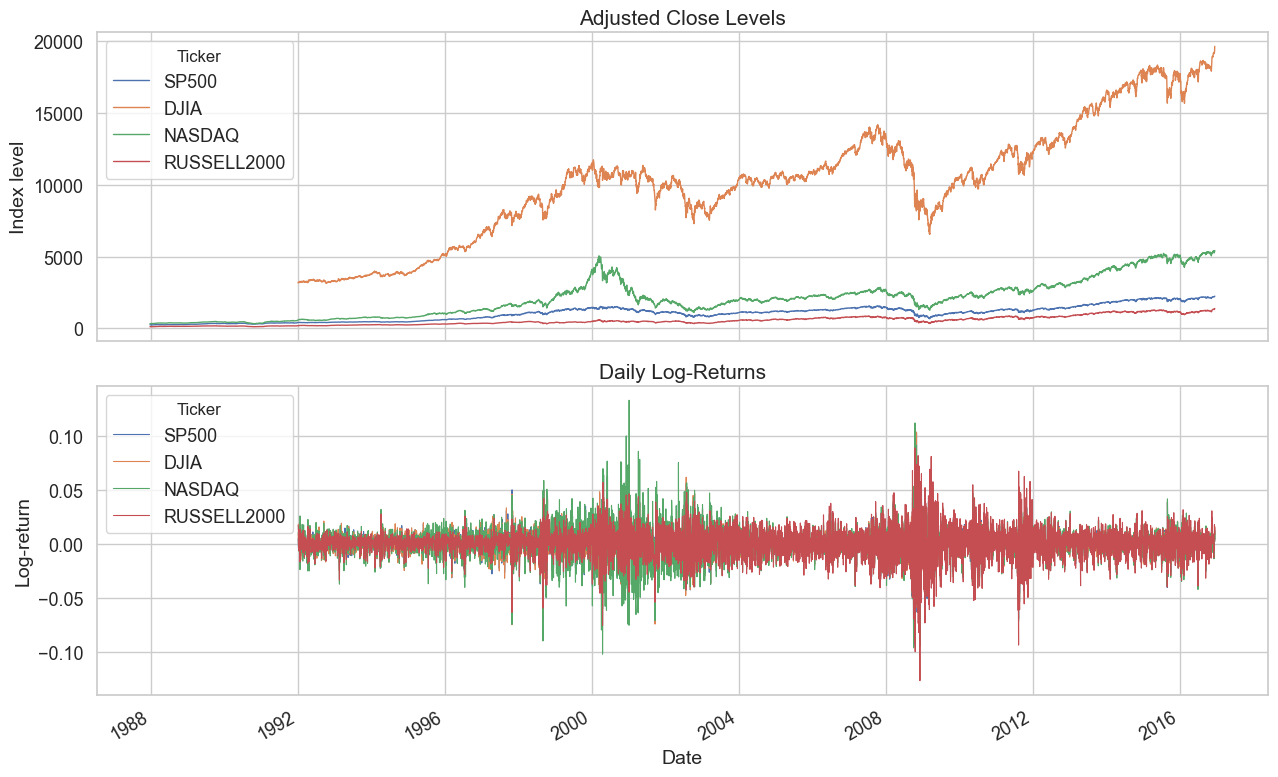
\includegraphics[width=0.80\textwidth]{figures/figure_cell7_out0.png}

\vspace{0.25em}
\footnotesize
Top: adjusted close levels for four indices. Bottom: daily log-returns used to form rolling 4D point clouds.
\end{frame}

\begin{frame}{Landscape Norm Time Series}
\centering
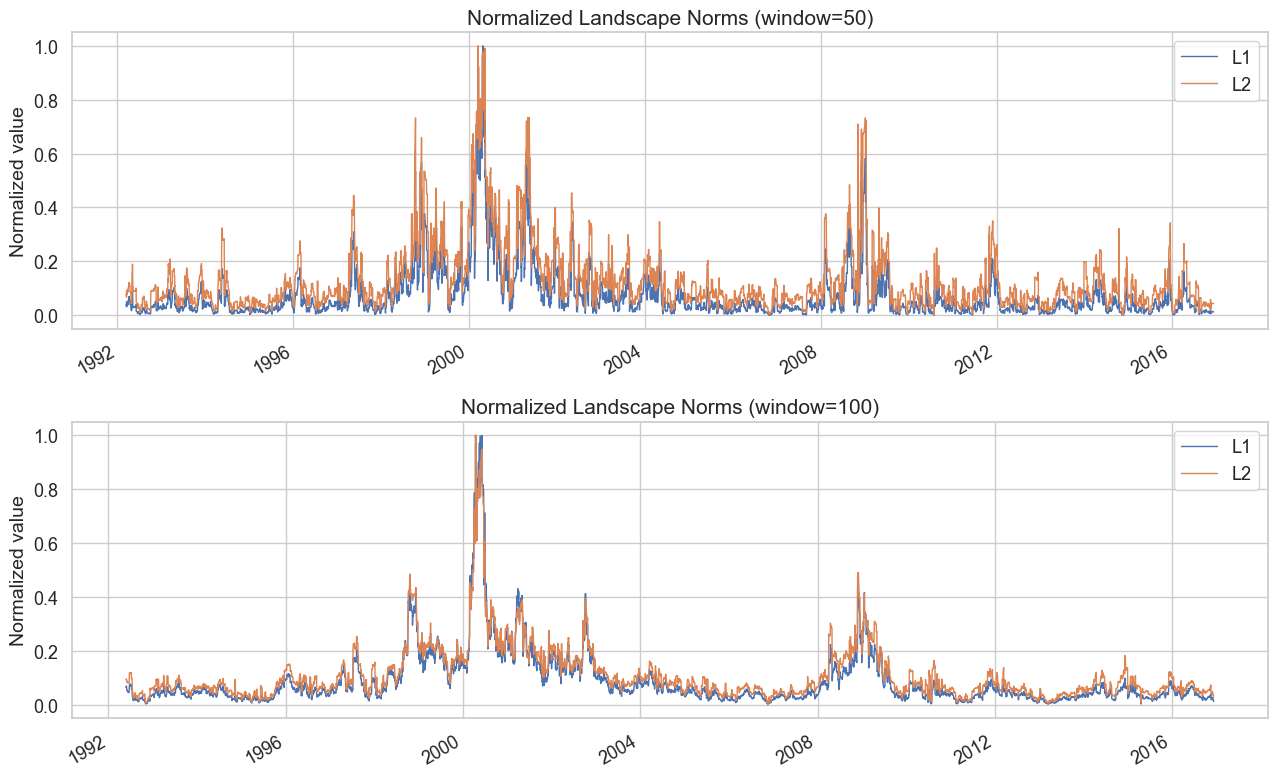
\includegraphics[width=0.80\textwidth]{figures/figure_cell13_out0.png}

\vspace{0.2em}
\footnotesize
\textbf{What this signifies:} higher \(L_1/L_2\) values indicate richer/less stable return-cloud topology; spikes cluster near stress regimes.
\end{frame}

\begin{frame}{Why the Output Is Meaningful}
\textbf{Interpretation logic}
\begin{itemize}
  \item Calm regimes: cloud geometry is tighter/more regular \(\Rightarrow\) smaller topological complexity.
  \item Transition-to-stress regimes: cloud deforms, dispersion rises, interactions become irregular.
  \item Persistent homology records this deformation through longer-lived \(H_1\) features.
  \item Landscape norms compress these geometric changes into a trackable scalar signal.
\end{itemize}
\end{frame}

\begin{frame}{Dot-Com vs Lehman}
\centering
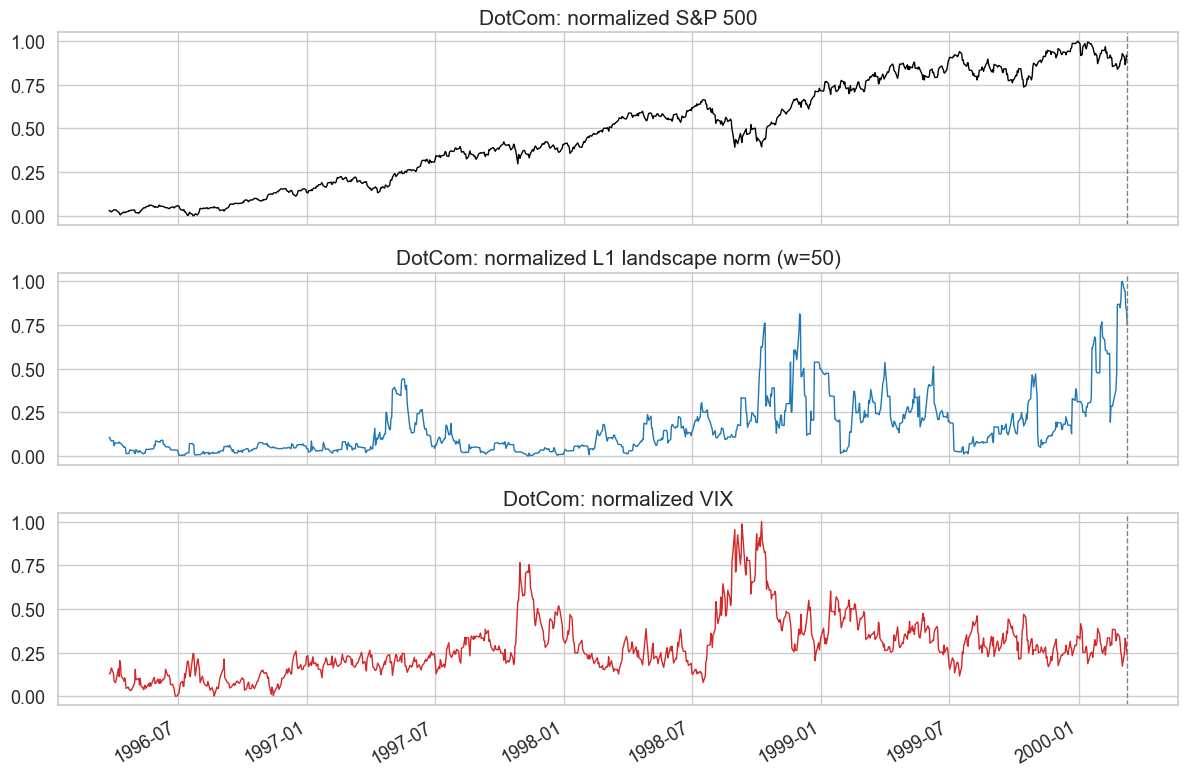
\includegraphics[width=0.48\textwidth]{figures/figure_cell15_out0.png}
\hfill
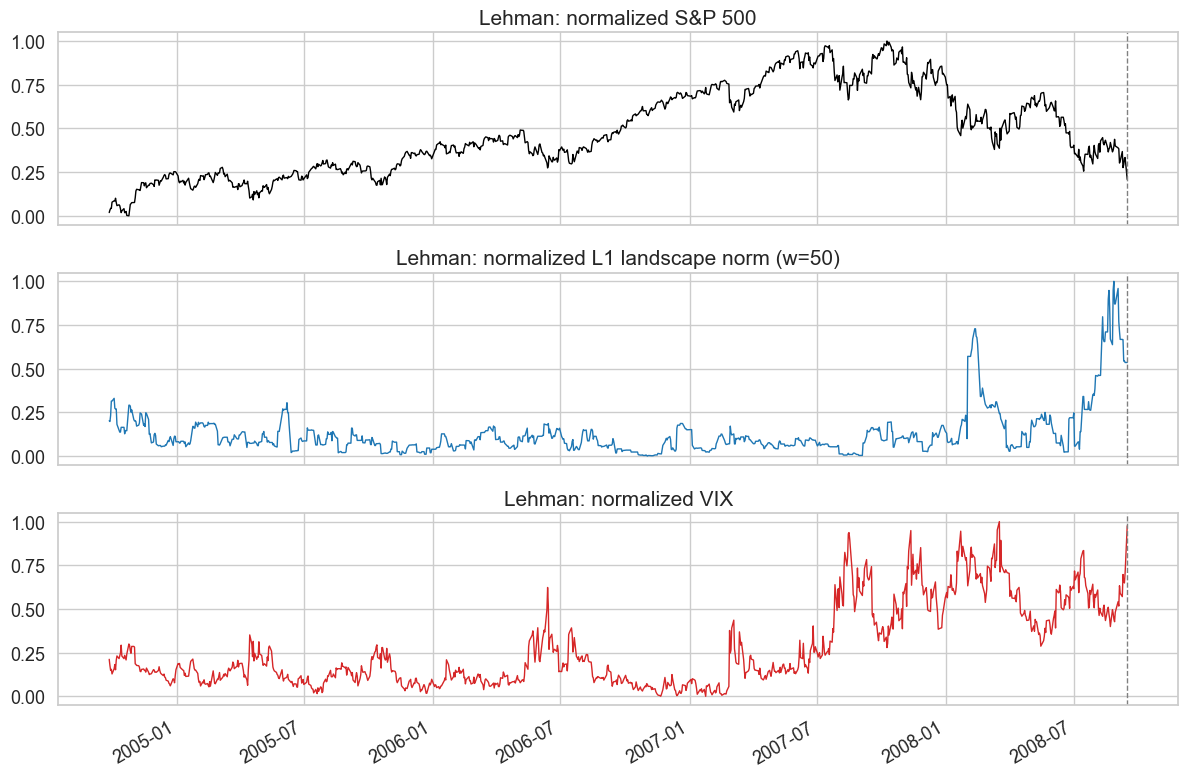
\includegraphics[width=0.48\textwidth]{figures/figure_cell15_out1.png}

\vspace{0.2em}
\footnotesize
Each panel shows normalized S\&P 500, normalized \(L_1\) landscape norm (\(w=50\)), and normalized VIX before event date.
\end{frame}

\begin{frame}{Quantitative Trend Diagnostics}
\small
\begin{table}
\centering
\begin{tabular}{>{\raggedright\arraybackslash}p{2.0cm}cc}
\toprule
\textbf{Event} & \textbf{Variance trend} & \textbf{Low-freq PSD trend} \\
\midrule
Dot-com & \(\tau=-0.223,\ p=1.44\times10^{-7}\) & \(\tau=-0.602,\ p=1.42\times10^{-45}\) \\
Lehman & \(\tau=0.888,\ p=4.36\times10^{-97}\) & \(\tau=0.691,\ p=1.40\times10^{-59}\) \\
\bottomrule
\end{tabular}
\end{table}

\normalsize
\textbf{Interpretation}
\begin{itemize}
  \item Lehman pre-window strongly supports increasing-risk narrative.
  \item Dot-com shows significant but opposite-direction trend in this run.
  \item This is an important replication nuance vs a uniform early-warning claim.
\end{itemize}
\end{frame}

\begin{frame}{Comparison to Course Methods}
\textbf{Methods common in course}
\begin{itemize}
  \item Volatility modeling, correlation structure, spectral/time-series diagnostics.
\end{itemize}

\textbf{What TDA adds}
\begin{itemize}
  \item Geometry of multivariate return clouds beyond second-order summaries.
  \item Potential sensitivity to structural regime change in cross-asset interactions.
  \item A complementary indicator family rather than a replacement.
\end{itemize}

\textbf{Practical framing}
\begin{itemize}
  \item Best used as part of a signal ensemble with standard risk indicators.
\end{itemize}
\end{frame}

\begin{frame}{Drawbacks and Limits}
\textbf{Methodological limitations}
\begin{itemize}
  \item \textbf{Parameter sensitivity:} window length, filtration scale, grid resolution.
  \item \textbf{Interpretability:} loop features are less intuitive than volatility/correlation.
  \item \textbf{Computational cost:} rolling persistent homology can be expensive.
  \item \textbf{Event heterogeneity:} not all crises produce the same trend direction.
\end{itemize}

\textbf{Empirical limitations}
\begin{itemize}
  \item Single market (US equities) and limited number of major crises.
  \item Potential data-vendor/library differences vs original implementation.
  \item Risk of overfitting narrative to a small set of historical events.
\end{itemize}
\end{frame}

\begin{frame}{Conclusions}
\textbf{What this replication supports}
\begin{itemize}
  \item End-to-end pipeline from paper is reproducible in modern Python.
  \item Topological landscape norms do capture stress periods, especially Lehman.
  \item TDA signals are useful as \emph{complements} to VIX and classical diagnostics.
\end{itemize}

\textbf{What remains open}
\begin{itemize}
  \item Robustness across assets, frequencies, and crisis definitions.
  \item Better statistical validation and out-of-sample warning evaluation.
  \item Translation into implementable risk-monitoring tools.
\end{itemize}
\end{frame}


\begin{frame}
\centering
\Large Thank you.
\vspace{0.6em}

\normalsize Questions?
\end{frame}

\end{document}
